\documentclass{ximera}

\addPrintStyle{..}


\begin{document}
	\author{Bart Lambregs}
	\xmtitle{De tweede wet van Newton}{}
%    \xmsource\xmuitleg

De eerste wet vertelt ons niet volledig wat er gebeurt wanneer op een lichaam een kracht werkt. Ze vertelt ons niet wat de relatie tussen kracht en beweging is. Dat doet de tweede wet.

Een bal waar je harder tegen schopt, krijgt een grotere snelheid mee en een pingpongballetje vliegt gemakkelijker weg dan een basketbal wanneer je er een tik tegen geeft. Als je het nader onderzoekt, door bijvoorbeeld verschillende krachten op een wagentje met eventueel steeds andere massa's te laten inwerken en de bijbehorende versnellingen te meten, merk je dat de versnelling recht evenredig is met de resulterende kracht en dat massa en versnelling omgekeerd evenredig zijn. M.a.w. $a\sim F/m$. Als bovendien een kracht zijdelings inwerkt op een bewegend voorwerp, dan merk je dat de baan afbuigt, in de richting van de kracht.

De eenheid van de grootheid kracht is de newton (symbool N). E\'en newton wordt gedefinieerd als de grootte van de kracht die een massa van \'e\'en kilogram een versnelling van \'e\'en meter per seconde kwadraat geeft.

Bovenstaande observaties, samen met de definitie van de eenheid van kracht, zitten vervat in de tweede wet van Newton, die een kwantitatieve relatie tussen kracht en versnelling poneert.

\begin{definition}
{\textbf{De tweede wet van Newton}} \nl

De versnelling van een voorwerp is recht evenredig met de erop inwerkende resulterende kracht en omgekeerd evenredig met de massa van het voorwerp. In symbolen:
\begin{equation*}
\vec{F}=m\vec{a}.
\end{equation*}
\end{definition}

\begin{remark}{De wet spreekt over de \emph{resulterende} kracht.} Het is de resulterende kracht die gelijk is aan $m\vec{a}$, niet zomaar een van de inwerkende krachten.
\end{remark}

\begin{remark}{Het gaat over de resulterende kracht die \emph{op} het voorwerp met massa $m$ wordt uitgeoefend en over de versnelling $a$ \emph{van} het voorwerp.} De krachten worden door andere voorwerpen op het voorwerp uitgeoefend. Het is niet dat het voorwerp een kracht `bezit' of een kracht op zichzelf kan uitoefenen.
	
\end{remark}

\begin{remark}{De formulevorm is een vectorvergelijking.} Zoals de kracht is, is ook de versnelling. Omdat de formule een vectorvergelijking is, is de gegeven formule equivalent met de componentsvergelijkingen:
	\begin{equation*}
		\vec{F}=m\vec{a}\quad\Leftrightarrow\quad
		\begin{cases}
			F_x=ma_x \\
			F_y=ma_y
		\end{cases}
	\end{equation*}
	De componentsvergelijkingen zijn in de praktijk handiger, er valt algebra\"isch mee te rekenen.
\end{remark}

De tweede bewegingswet geeft een verband tussen de oorzaak van een beweging (de resulterende kracht) en de versnelling van de beweging.

De formulevorm van de tweede wet ziet er misschien gemakkelijk uit maar is in al haar eenvoud \emph{immens} krachtig. De wetmatigheid verklaart alle mechanische bewegingen; als we de krachten kennen, kennen we de versnelling van het voorwerp en kunnen we (althans op zijn minst in theorie) de baan van het voorwerp bepalen.

In feite zit de eerste wet vervat in de tweede. Toch blijven we hem gebruiken, vooral om het concept traagheid te benadrukken.

\begin{denkvraag*}{}
	Waar en hoe in het filmpje van Wile E. Coyote en de Road Runner wordt de tweede wet van Newton met de voeten getreden?
	\begin{center}
		\youtube{hvjAr6cHUVM}
	\end{center}
\end{denkvraag*}

\begin{exercise}
	Een massa van \SI{2,0}{kg} bevindt zich in een lift aan een dynamometer. Die laatste duidt een kracht van \SI{10}{N} aan. Welke beweging voert de lift uit?

	\begin{minipage}[c]{.8\linewidth}
	\begin{multipleChoice}
		\choice[correct]{De lift beweegt naar omlaag met een versnelling van \SI{5,0}{m/s^2}.}
		\choice{De lift beweegt naar omhoog met een versnelling van \SI{5,0}{m/s^2}.}
		\choice{De lift beweegt naar omlaag met een constante snelheid.}
		\choice{De lift beweegt naar omhoog met een constante snelheid.}
	\end{multipleChoice}
	\end{minipage}
	\hfill
	\begin{minipage}{.15\linewidth}
	\begin{image}
		%  \vspace*{0pt}   % ensure top alignment
		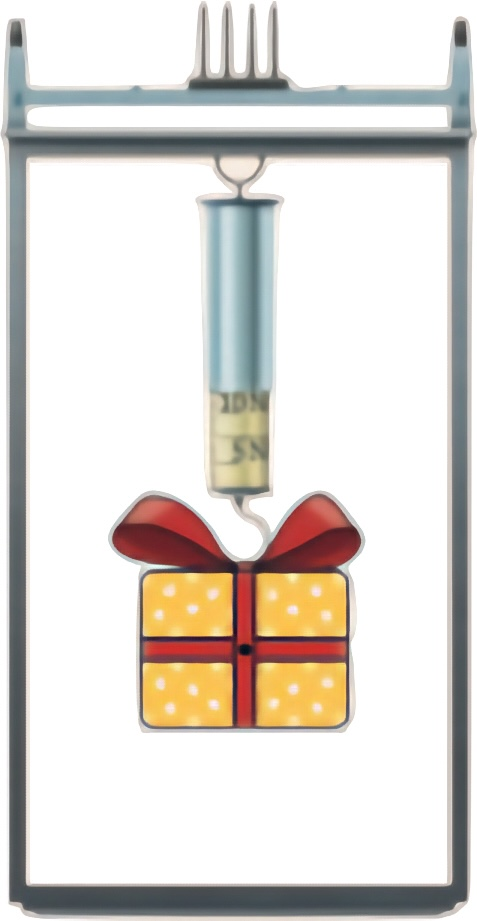
\includegraphics{FV_9p143}%
	\end{image}
	\end{minipage}
\end{exercise}

\begin{exercise}
	Op een luchthaven trekt een vrouw haar koffer met een constante snelheid voort. Het handvat maakt een hoek $\theta$ met de horizontale. De massa van de koffer is \SI{10,5}{kg}. De vrouw trekt volgens de richting van het handvat met een kracht van \SI{25,0}{N} terwijl de grootte van de wrijvingskracht op de valies \SI{11,0}{N} bedraagt.

	\begin{minipage}[c]{.7\linewidth}
		\begin{enumerate}
			\item Teken het krachtendiagram van de koffer.%\footnote{Teken en benoem met andere woorden alle krachten die op de koffer aangrijpen. Laat de krachten aangrijpen in het zwaartepunt van de koffer.}
			\item Bepaal de hoek $\theta$ tussen het handvat en de horizontale.
			\item Bepaal de normaalkracht die de grond op de koffer uitoefent.
		\end{enumerate}
	\end{minipage}
	\hfill
	\begin{minipage}{.2\linewidth}
	\begin{image}
			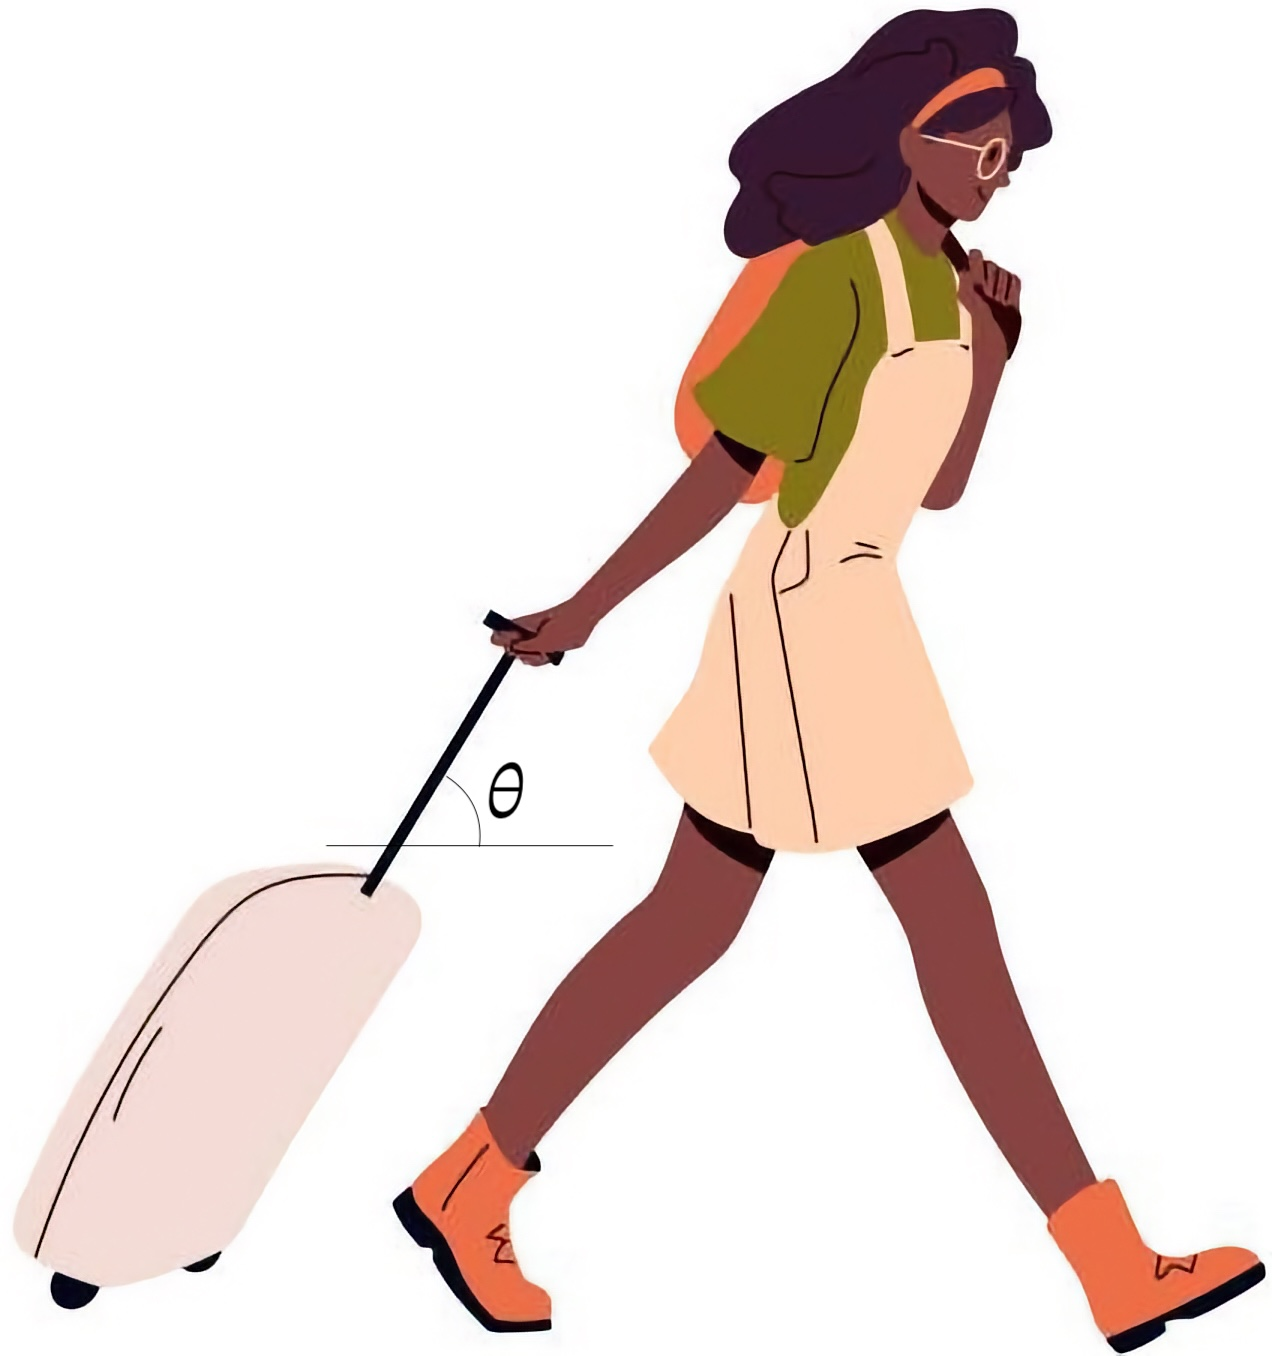
\includegraphics{istockphoto-1430278348-612x612_theta}%
	\end{image}
	\end{minipage}
	\begin{oplossing}
	% 	\begin{enumerate}
	% \item [\textit{gegeven}]
	% \begin{tabular}[t]{lcl}
	% $m$ &$=$& \SI{10,5}{kg}\\
	% $F$ &$=$& \SI{25,0}{N}\\
	% $F_w$ &$=$& \SI{11,0}{N}
	% \end{tabular}
	% \item [\textit{gevraagd}]
	% $\theta$, $F_n$
	% \item [\textit{oplossing}]
	De snelheid is constant zodat volgens de horizontale richting de versnelling nul is. De component van de trekkracht volgens deze richting moet dan ook even groot zijn als de wrijvingskracht:
	\begin{eqnarray*}
		F\cos{\theta}&=&F_w\\
		&\Updownarrow&\\
		\theta &=& {\rm bgcos}\left(\frac{F_w}{F}\right)\\
		&=& \SI{1,16}{rad}\qquad =\SI{64}{\degree}
	\end{eqnarray*}
	Ook volgens de verticale richting is de versnelling nul zodat\footnote{Als je expliciet het gevraagde in functie van de gegevens wil zetten, moet je de $y$-component van de trekkracht met de stelling van Pythagoras berekenen. De uitkomst is dan $F_n=mg-\sqrt{F^2-F_w^2}$.}:
	\begin{eqnarray*}
		F\sin{\theta}+F_n&=&F_z\\
		&\Updownarrow&\\
		F_n &=& mg-F\sin{\theta}\\
		&=& \SI{83}{N}
	\end{eqnarray*}
	%\end{enumerate}
	\end{oplossing}
\end{exercise}

\begin{exercise}
	In de laadruimte van een vrachtwagen hangt een slinger aan het plafond vast. Doordat de vrachtwagen met een constante versnelling optrekt, maakt het touw van de slinger een hoek van $\SI{37}{\degree}$ met de verticale. 
	
	\begin{image}
		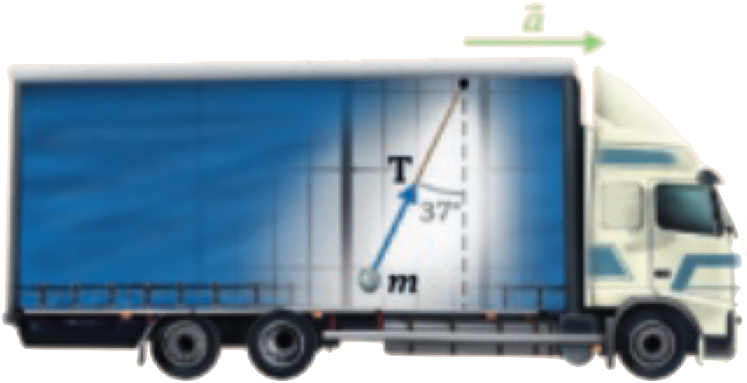
\includegraphics[width=.62\textwidth]{FV_8p153}
	\end{image}
	
	Bepaal de grootte van de versnelling van de vrachtwagen.
\end{exercise}

\begin{exercise}
	Onder invloed van een kracht $\vec{F}$ beweegt een blok met constante snelheid over een ruw horizontaal oppervlak. De krachten op de figuur hebben de juiste ori\"entatie maar niet noodzakelijk de juiste grootte. Welke van de volgende relaties tussen $\vec{F}$, $\vec{F}_w$, $\vec{F}_z$ en $\vec{F}_n$ moet in ieder geval waar zijn?

	\begin{minipage}{0.6\textwidth}
	\begin{multipleChoice}
	\choice{$F_w=F$ en $F_n=F_z$}
	\choice[correct]{$F_w<F$ en $F_n<F_z$}
	\choice{$F_w=F$ en $F_n>F_z$}
	\choice{$F_w<F$ en $F_n=F_z$}
	\end{multipleChoice}
	\end{minipage}
	\hfill
	\begin{minipage}{0.35\textwidth}
	\begin{image}
			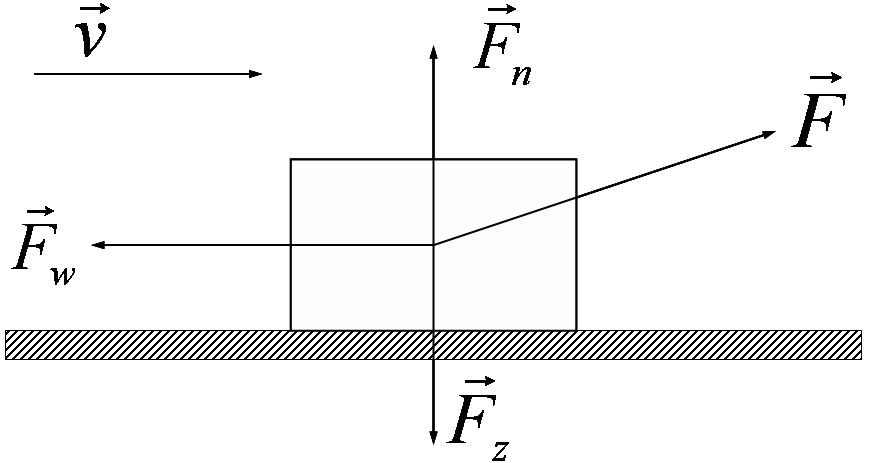
\includegraphics{blok_horizontvlak}
	\end{image}
	\end{minipage}

	\begin{oplossing}
	We ontbinden de kracht $\vec{F}$ in zijn twee componenten volgens de horizontale en verticale richting: $\vec{F}_x,\vec{F}_y$. Aangezien het blok in de verticale richting niet versnelt, moet $F_z=F_n+F_y$ of $F_n<F_z$.
	\end{oplossing}
\end{exercise}

\end{document}
